% !TeX spellcheck = en_US
\documentclass[12pt, oneside]{book}              % Book class in 11 points
\usepackage{amsmath, amsthm, amssymb}
\usepackage[english]{babel}
\usepackage[utf8]{inputenc}
\usepackage{cancel}
\usepackage{graphicx}
\usepackage{hyperref}% add hypertext capabilities
\setlength{\parskip}{4mm}

% For several graphics per figure
\usepackage{caption} %[caption=false]
\usepackage{subfigure}

% For centering elements in tables
\usepackage{array}

% For multirows and multicolumns in tables
\usepackage{multicol}
\usepackage{multirow}

% Epigraph
\usepackage{epigraph}

% List package (useful to write codes)
\usepackage{color}
\definecolor{mygreen}{rgb}{0,0.6,0}
\definecolor{mygray}{rgb}{0.5,0.5,0.5}
\definecolor{mygray2}{rgb}{0.9,0.9,0.9}
\definecolor{mymauve}{rgb}{0.58,0,0.82}
\usepackage{listings}
\lstset{
basicstyle=\small\tt,
breaklines=true,
commentstyle=\color{mygreen}\small,
keywordstyle=\color{blue}\small,
stringstyle=\color{mymauve}\small,
numbers=left,
numberstyle=\small\color{mygray},
backgroundcolor=\color{mygray2},
showstringspaces=false,
tabsize=3
}

% Appendix
\usepackage[toc,page]{appendix}


%\oddsidemargin 0.4cm \evensidemargin 0.4cm \topmargin 0.0cm
%\textwidth 15.7cm \textheight 22.0cm \headsep 1.2cm \footskip 1.0cm

\title{\bf Documentation of the project: \\ ISR jet tagging}
\author{\textbf{Author:}\\ Andr\'es Felipe Garc\'ia Albarrac\'in \\ \\ \textbf{Advisor:} \\ Juan Carlos Sanabria, Ph.D.}
\date{\today}

\begin{document}                        % End of preamble, start of text.
	\frontmatter                            % only in book class (roman page #s)
	\maketitle                              % Print title page.
	\tableofcontents                        % Print table of contents
	\mainmatter                             % only in book class (arabic page #s)

\chapter{Introduction}

During the last semester of 2014, I made my Undergraduate Thesis Project entitled 
``\textit{Design of algorithms to identify high momentum Initial State Radiation 
(ISR) Jets in proton – proton collision events}'', under the supervision of Juan
Carlos Sanabria, Ph.D.. As the name suggests, the project consisted in the proposal
of an algorithm to identify ISR jets. Due to the promising results, I was employed 
during the first semester of 2015 under the charge ``Joven Investigador'' of 
COLCIENCIAS in order to improve the initially obtained results. Throughout this
time, several codes and programs were developed. To encourage the continuation of
this project, this report has been written with a summary of all the technical 
work done so far.

In practical matters, one of the main drawbacks of Quantum Field Theory (QFD) is 
the inherent difficulty of its calculations. Feynman diagrams are not easy to solve
and specially when high orders are involved. Consequently, the usage of algorithms
and computer simulations have played an important role in the prediction of 
numerical results thanks to the great calculation power of modern computers. Several
programs have been written with this purpose and today there exists a machinery
which combines QFD, statistical models and Monte Carlo methods to reproduce High
Energy Physics experiments.

In this project, three of those programs were used: 
MadGraph 5.2 (MadEvent)~\cite{Alwall:2014hca}, Pythia 8.2~\cite{Sjostrand:2014zea} 
~\cite{Sjostrand:2006za} and Delphes 3.2~\cite{deFavereau:2013fsa} with the aim of 
simulating proton - proton collision events. The description of those programs and
their particular purposes in the project are described in chapter 
\ref{cha:Simulation_chain}. In addition, chapter \ref{cha:Simulation_chain}
includes the explanation of the codes and the scripts that were developed
both to integrate those programs, and to run the simulations under specific conditions.

In despite of the fact that those simulations demanded a huge amount of computational
time, they just served as inputs of the algorithms written throughout the project,
which contain the main proposed analysis and ideas. Altogether, four algorithms
were elaborated. Each of them are explained in chapter 3, where their documentation
and an overall description are presented. 

Finally, chapter four includes a brief description of some software tools that
were introduced to the project. Specifically, this project used C++ codes which
included root libraries instead of root macros. This transition reduced the 
execution time of the algorithms six times. Additionally, the development 
environment \emph{Eclipse} was also introduced, which made easier the programming
process. Overall, these tools dramatically improved the technical work of the project.

\chapter{Simulation chain} \label{cha:Simulation_chain}

\epigraph{\textquotedblleft \textit{Divide et impera}\textquotedblright, \\ \textquotedblleft
Divide and conquer\textquotedblright}{Philip II of Macedon}

At first glance, it is not clear why it is necessary to use three programs at the
simulation stage instead of just one. The answer is quite simple: each one of those
programs has been developed to run a specific task in the simulation process, and 
therefore, each one has been optimized to do so as accurate and fast as possible. 
While MadGraph and Pythia are responsible for the simulation of high energy collision's 
Physics, Delphes takes the final state particles produced by the former programs, and
determines what would be the corresponding response of a detector. This scheme is
useful as it maintains the detector apart from the main calculations of the simulation.
Additionally, it makes the change of experiment parameters as simple as modifying
Delphes execution specifications.

As presented before, MadGraph and Pythia handle the Physics of the collision. Again,
there is more than a single program for this task, and now the reason to use two programs lies on the
limits of the theoretical models. At the very first moment of the collision when
the Energy Density of the System is high enough, perturbative Quantum Chromo-Dynamics
(pQCD), Quantum Electro-Dynamics (QED) and ElectroWeak Theory are the most accurate models
known so far. MadGraph, and specifically MadEvent, use them to calculate the transverse
sections of a particular channel defined by the user. From this calculation and the Monte 
Carlo models, it randomly establishes the kinematic variables of the resulting particles
of the collision.

Once the energy density of the collision has been reduced significantly, the models used
by MadGraph are not valid, and then Pythia appears in the scene. The particles resulting
from MadGraph are taken by Pythia, which makes the evolution to a multi-hadronic final
state ~\cite{Sjostrand:2014zea}. The task run by Pythia involves the usage of Monte
Carlo techniques to simulate hadronization, decays and showers. Finally, the particles
obtained at the end of the Pythia simulation are the inputs for the Delphes simulation.

Although the usage of several programs for the simulation means better results, it also
implies the challenge of connecting them. This task has already been done inside the MadGraph
package, which connects MadEvent + Pythia 6 + Delphes / PGS\footnote{\textit{Pretty 
Good Simulation}, PGS, is another program for detector simulation}. However, the version
of Pythia included there (v.6) is old and does not offer the possibility of controlling 
ISR emissions as the last one (v.8) does. As ISR emissions were the main focus of the 
project, it was convenient to use Pythia 8 instead of Pythia 6 and therefore to develop
the integration of MadGraph 5.2 with Pythia 8.2 and Delphes 3.2.

Throughout this chapter, the codes and scripts written to achieve the simulation will
be explained. One section is devoted to each program and another one presents the
script that connects the three programs. Finally, the last section of this chapter
presents a simulation example where such script is used.
%Finally, the last section of this chapter
%presents the procedure known as Matching between MadGraph and Pythia, which ensures that
%the physics calculations made by each program correspond to the Energy scale that
%each one of them should handle.

\section{Usage of MadGraph 5.2} \label{sec:MadGraph}

The most basic procedure to simulate collision events using MadGraph is by means of its
executable program. Follow the next steps to run a set of simulations of the channel
$ p\ p\ \to t\ \tilde{t} $. It is important that MadGraph has been correctly installed
\footnote{A full set of instructions to install MadGraph and other High Energy Physics
programs can be found at \url{http://goo.gl/vigBdj}}.

\begin{enumerate}
\item In the folder where MadGraph has been installed, type:  
\\ \texttt{./bin/mg5\_aMC}
\item Once MadGraph has been initialized, import the Standard Model parameters:
\\ \texttt{import model sm}
\item Generate the event $ p\ p\ \to t\ \tilde{t} $:
\\ \texttt{generate p p > t t$ \sim $}
\item Create an output folder where all the simulation files will be saved, in this case
test\_t\_tbar:
\\ \texttt{output test\_t\_tbar} 
\item Launch the Feynman diagrams production:
\\ \texttt{launch -m}
\\ and select the number of cores you want to use for the simulation
\item Turn off Pythia and other programs\footnote{This project uses the last version 
of Pythia (8.2) instead of the sixth version that uses MadGraph}. You can switch 
off and on by typing the number before the program (type 1 to toggle pythia, for instance).
Then, press enter.
\item Modify the \texttt{run\_card.dat} file by typing 2. Write \texttt{:32} and press
enter to go to line 32, then type \texttt{i} and press enter to modify the file. Change
the number of events from 10000 to 1000. Press \texttt{Esc} and write \texttt{:wq} to
write and quit.
\item Press enter to run the simulation

\end{enumerate}

Although simple, the latter approach is not the best as it requires the user interaction
several times to configure the simulation, which is not desirable when more than a single 
simulation will be performed. In such situations, all the configuration parameters
can be defined trough an input file. For the previous example, the input file would be:

\noindent \texttt{import model sm
\\generate p p > t t\~
\\output test\_t\_tbar -f
\\launch -m
\\2
\\pythia=OFF
\\Template/LO/Cards/run\_card.dat
\\models/sm\_v4/param\_card.dat}

\noindent where 2 corresponds to the number of cores used in the simulation, 
\texttt{run\_card.dat} is the default file of MadGraph and \texttt{param\_card.dat} 
contains the Standard Model parameters and values. Here, these two files correspond
to the default ones that MadGraph provide. In order to use another set of 
configuration parameters, the files should be copied to another location
and modified according to desired simulation conditions.

The input file may be saved as \texttt{mg5\_input.mg5} and the simulation can be
executed as:

\noindent \texttt{./bin/mg5\_aMC -f mg5\_input.mg5} \footnote{Observe that it is
supposed that \texttt{mg5\_input.mg5} is localed at the MadGraph folder and that
the command is run from the same directory. If not, the execution instruction and
the input file should contain the full path accordingly.}

As a result of the simulation by MadGraph, the output folder contains several 
folders with all the information related to the simulation. The folder 
\texttt{Cards} for instance, contains some parameter cards used in the simulation,
while the folder \texttt{HTML}, and specially the file \texttt{info.html} present
the Feynman diagrams created by MadGraph. The events resulting from the simulation
are found in the folder \texttt{Events/run\_01} in the form of two files: a root 
file called \texttt{unweighted\_events.root} and a compressed Les Houches Event file
with name \texttt{unweighted\_events.lhe}.

\section{Usage of Pythia 8.2} \label{sec:Pythia8}

The simulation carried out by MadGraph is now passed to Pythia, which takes the
file \texttt{unweighted\_events.lhe} as input. Pythia uses the information 
contained in such file to develop the hadronization, and produces another file
with the kinematic variables of the resulting particles. The task performed by
Pythia can be summarized in the Black Box of Fig. \ref{fig:Black_box_pythia}, 
where in addition to the file produced by MadGraph, a plain text file with 
extension \texttt{.cmnd} is passed by parameter to configure the simulation.

\begin{figure}[h]
\centering
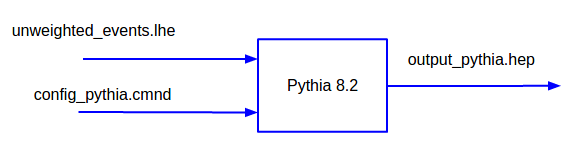
\includegraphics[width=0.7\linewidth]{Imags_Doc/Black_box_pythia}
\caption{}
\label{fig:Black_box_pythia}
\end{figure}

The functionality of the black box of \ref{fig:Black_box_pythia} is done by
a program written in C++, which is based on the examples provided by Pythia 
developers ~\cite{Sjostrand:2006za}. The code is called \texttt{hadronization02.cc}, 
was written in C++ and can be found at Appendix \ref{App:hadronization02.cc}.
It performs specific requirements for this project that will be mentioned soon. 
Before presenting the operations performed by the program, it is convenient 
to describe how this code should be compiled and used. 

\subsection{Code Usage}\label{sub:Code_usage}

To use \texttt{hadronization02.cc}, it is necessary to have installed 
Pythia\footnote{Again, information to install Pythia 8.2 and HepMC can be 
found at \url{http://goo.gl/vigBdj}} and StdHep\footnote{StdHep can be 
downloaded from \url{http://cepa.fnal.gov/psm/stdhep/getStdHep.shtml}.
It is enough to type \texttt{make} to install it}~\cite{Garren-StdHep}.
Once installed, go to the \texttt{examples} folder located at the Pythia
directory \footnote{If \texttt{examples} is not exactly there, it may 
be in \texttt{share/Pythia8}}.
Inside such folder, copy the code \texttt{hadronization02.cc} and then 
modify the \texttt{Makefile} in order to compile it. It is enough to insert
the following lines at the beginning of the \texttt{Makefile}:

\lstinputlisting[language=make]{Codes/Make_first_part}

\noindent changing \texttt{<STDHEP Directory>} in line 2 by the local
installation directory of StdHep. Furthermore, these other lines should
be included at the end of the \texttt{Makefile}:

\lstinputlisting[language=make]{Codes/Make_second_part}

After doing so, the code is compiled by typing on terminal:

\texttt{make hadronization02}

As a result, the executable file \texttt{hadronization02} is created in 
the current folder. It may be copied and used in other directory.
The instruction to run this program is:

\texttt{./hadronization02 input.cmnd [output.hep]}

\noindent where \texttt{input.cmnd} is the full name (with the path) of 
the configuration file, and \texttt{output.hep} is an optional parameter
that corresponds to the name of the output file.

Continuing with the $ t\ \tilde{t} $ production example of the previous
section, the following file may be saved as \texttt{input.cmnd} and
used as input of the Pythia simulation:

\lstinputlisting{Codes/input_pythia.cmnd}

Each line of this file is a different command, each of which is described after
the exclamation mark character \textquoteleft!'. As it can be seen, 1000 
events are hadronized, the file \texttt{unweighted\_events.lhe} from 
MadGraph is read, and only ISR emissions are allowed.

\subsection{The code}\label{sub:Pythia_code}

Having explained the procedure to compile and use the hadronization program, 
this subsection presents the code and what it does. As stated before, the code
can be found in the Appendix \ref{App:hadronization02.cc} and also, in the 
repository of the project: \url{https://github.com/andresfgarcia150/ISR_tagging_project},
at the folder \texttt{/Codes/Simulation/Pythia\_Codes/}, where the modified
Makefile is also included.

Overall, the code can be described in terms of two procedures: the configuration
and the execution of the simulation. The first of them, that corresponds to
lines 76 - 106 in Appendix \ref{App:hadronization02.cc}, establishes all the
parameters needed for the simulation. It starts with the definition of some Strings
to be used by the StdHep methods, and an object of class \texttt{Pythia} in line 82.
Then, in lines 84-93, the names of the input file (\texttt{.cmnd} file) and the 
output file are read from the execution instruction by means of \texttt{**argv}.
Next, lines 95-98 define some variables to control the hadronization: 
\texttt{nEvent} corresponds to the number of events to be hadronized, while
\texttt{nAbort} and \texttt{iAbort} are the maximum and current numbers of 
allowed events that present an error. Finally, the simulation configuration 
ends with some necessary functions to handle StdHep files (lines 100-102) and
with the definition of an object of the class \texttt{MyUserHooks}.

The latter definition is extremely important for this project as it contains
the restriction on the ISR emission. The object defined in line 105 belongs to
the class \texttt{MyUserHooks}, which is written at the beginning of the code 
(lines 37-67). This class, in turn, inherits from \texttt{UserHooks} and just
two of its methods are re-written: \texttt{canVetoISREmission()} and 
\texttt{doVetoISREmission()}. Each time an ISR emission is produced during
the simulation of an event, the first of those methods stops the simulation
and executes the second one, which counts the number of ISR partons produced
so far and veto all the emissions in case that already exits one. This way, 
only one (or zero) ISR parton is produced in each event. 

With the definition of the pointer \texttt{myUserHooks} and its inclusion in
the object \texttt{pythia}, the configuration stage finishes. Then, the execution
starts by initializing the simulation at line 109. Basically, the simulation consists
of the \textit{for} loop of lines 111-125, where each iteration corresponds to
the generation of a new event through the call of method \texttt{pythia.next()}.
Observe that if the latter method returns \texttt{false}, either pythia has reached the
end of the input file (from MadGraph), or an error has happened and the execution
should stop if the maximum number of errors is reached. Once this has been verified,
each cycle ends by writing the event in the output \texttt{.hep} file.

After the simulation has been completed, the StdHep file is closed 
in line 127, some statistics of the simulation are published (line 128) and the
pointer  \texttt{MyUserHooks} is deleted. These lines conclude the code that 
develops the hadronization process.

\subsection{Pythia ntuple generation} \label{sub:Pythia_ntuple}

Although the file produced by the latter code is passed directly to Delphes, it
cannot be read by ROOT. Therefore, it is necessary to develop a conversion
from \texttt{.hep} to \texttt{.root}, which is performed by \texttt{ExRootAnalysis}.
After having it properly installed, go to the installation directory and
run the executable file \texttt{ExRootSTDHEPConverter} by typing:

\texttt{./ExRootSTDHEPConverter output\_pythia.hep output\_pythia.root}

\noindent where \texttt{output\_pythia.hep} is the full path name of the
file produced by the hadronization code and \texttt{output\_pythia.root} is
the output \texttt{ntuple}. This procedure makes possible the reading of 
the pythia simulation when executing C++ codes with Root libraries.

\begin{center}
***
\end{center}

To summarize, it has been shown how to carry out simulations with MadGraph and
Pythia 8.2. As a result of the simulation of MadGraph, the file 
\texttt{unweighted\_events.lhe} is produced. Pythia receives that file as
parameter and creates the file \texttt{output\_pythia.hep}. To complete the 
simulation process, the next section will introduce Delphes, that takes the file
generated by Pythia and performs the detector simulation.

\section{Usage of Delphes 3.2} \label{sec:Delphes}

Because High Energy Experiments such as the Compact Muon Solenoid (CMS) and 
A Toroidal LHC ApparatuS (ATLAS) are already created and there is not much 
we can do to modify them, the simulation of those detectors is a simple task.
To use Delphes, for instance, it is enough to have it installed and use
the existent cards.

For the CMS simulation of the $ t\ \tilde{t} $ production example that
has been used throughout this chapter, go to the Delphes installation
directory and use the execution file \texttt{DelphesSTDHEP}. To do so,
type on the terminal:

\texttt{./DelphesSTDHEP cards/delphes\_card\_CMS.tcl output\_delphes.root output\_pythia.root}

\noindent taking care that each one of the parameters should be replaced
by the full path name of each file. With this instruction, 
\texttt{delphes\_output.root} is generated and the files: 
\texttt{output\_pythia.root} from the Pythia simulation, and
\texttt{delphes\_card\_CMS.tcl} with CMS experiment specs are taken
as inputs.

\begin{center}
***
\end{center}

Delphes is the last link of the simulation chain and at the end,
there are three ntuples to be used by the analysis algorithms:

\begin{enumerate}
\item \texttt{unweighted\_events.root}: The ntuple produced by MadGraph.
It contains the kinematic variables of the hard partons resulting from
Feynman diagram calculations.
\item \texttt{output\_pythia.root}: The ntuple generated by Pythia. It
contains the information of all particles after hadronization and showering.
In addition to final state particles, this file also stores a copy of all
intermediate particles created during the hadronization process. It should
be convenient to check the documentation about the particles' status 
~\cite{Sjostrand:2006za} for more information.
\item \texttt{output\_delphes.root}: The ntuple created by Delphes.
It presents the simulation information as a detector should report, i.e.
in terms of jets, photons, electrons, etc.
\end{enumerate}

These three files are the final result of the simulation and as it will
be presented later, the latter two will be used in this project. The
procedure to obtain them has been presented and despite being straightforward,
it is cumbersome as it requires several times the user intervention.
Simulating would be a tedious task when several runs need to be executed such as
the situation that this project deals with. Therefore, it was necessary
to create an script that involved the three steps of the simulation. This
script, originally written by Diego A. Sanz\footnote{\url{d-sanz@uniandes.edu.co}}
to run MadGraph alone, was modified to include Pythia 8.2 and Delphes 3.2,
and it is the topic of the next section.

\section{Integration of MadGraph 5.2 + Pythia 8.2 + Delphes 3.2}

To integrate MadGraph 5.2 with Pythia 8.2 and Delphes 3.2 two scripts were
written, which can be found in the Appendix \ref{App:scripts} and in the 
repository of the project\footnote{\url{https://github.com/andresfgarcia150/ISR_tagging_project}}
at the folder \texttt{Codes/Simulation/MG\_pythia8\_delphes\_parallel}.
Those scripts allow parallel simulations taking advantage of the
computing capabilities of the machine where the user is working.

Basically, the first script sets all the parameters needed for
the simulation, which is executed by the second script. Thus, the
user needs to modify all the variables in \texttt{config\_Integration.ini}
according to the local installation directories and the folders
where the run and param cards are located. After doing so, it
is sufficient to execute \texttt{script\_Integration.sh} in order to run
the simulation:

\texttt{./script\_Integration.sh}

\noindent This way, there is not risk of accidentally changing the execution
script.

Although both scripts are well documented, it is worth mentioning
some words about them:

\begin{itemize}
\item Because the scripts execute parallel simulations, it
is necessary to specify two folders where they will be saved:
\texttt{EVENTSFOLDER} is the name of the head directory where all
simulations will be saved, and \texttt{NAMESUBFOLDER} is the generic
name of the folders that contain each simulation and that are 
located at \texttt{EVENTSFOLDER}. Thus, simulation \#3 is saved in 
\texttt{EVENTSFOLDER/NAMESUBFOLDER3}.

\item In total, each execution of \texttt{script\_Integration.sh} run
simulations from \texttt{INIRUN} to \texttt{ENDRUN}. Each of them
consists of \texttt{NUMEVENTSRUN} events and its seed is the simulation
number.

\item Because MadGraph can develop some parallel calculations, 
\texttt{CORESNUMBER} is the number of cores devoted to each MadGraph
run. Be aware that the total number of parallel runs times \texttt{CORESNUMBER}
needs to be less or equal than the number of cores of your machine. 
Once MadGraph has been executed, only one core of \texttt{CORESNUMBER}
is used to run Pythia and Delphes, because they only manage
one thread.

\item There are two sequences inside \texttt{script\_Integration.sh} . The
first one copies and modifies the run and param cards according to
each simulation (it changes the seed, for instance). At the end of this
sequence, those copies are located at the folders \texttt{/RunCards/} and
\texttt{/ParamCards/} inside \texttt{EVENTSFOLDER}. When configuring
\texttt{config\_Integration.ini}, it is extremely important to use the 
templates of the files:
\begin{itemize}
\item \texttt{run\_card.dat}
\item \texttt{mgFile.mg5}
\item \texttt{input\_pythia.cmnd}
\end{itemize}
provided at the folder \texttt{Codes/Simulation/MG\_pythia8\_delphes\_parallel}
\texttt{/RunCard\_Template} of the repository, as the script looks for
certain variables defined in such templates and replace them with
the specific parameters of each simulation.

\item The second sequence inside \texttt{script\_Integration.sh} runs the
simulations. As it can be verified in Appendix \ref{sub:Execution_script},
it:
\begin{enumerate}
\item Runs Madgraph
\item Uncompresses the .lhe.gz file produced by MadGraph
\item Executes Pythia
\item Executes Delphes
\item Makes the conversion \texttt{output\_pythia.hep -> output\_pythia.root}
\item Remove unnecessary files.
\end{enumerate}

Contrary to the first sequence, this second one is run in parallel using
the program Parallel ~\cite{Tange2011a}.
\end{itemize}

\section{Example of the integration scripts}\label{sec:Example_script}

The example that was presented when each one of the programs was explained
will now be repeated with the scripts introduced in above. Follow the next 
instructions to simulate 100000 events of the channel $ p\ p\ \to\ t\ \tilde{t} $,
where additionally one $ W $ boson resulting from the tops' decays
is required to decay hadronically while the other is forced to a leptonic decay:

\begin{enumerate}
\item Install the three programs and compile the code \texttt{hadronization02}
of Pythia.
\item Download the folder \texttt{MG\_pythia8\_delphes\_parallel} from the
repository of the project.
\item Open the file \texttt{config\_Integration.ini} and write all the installation
folders in front of the corresponding variables. Use the path of the downloaded folder
\texttt{RunCard\_Template} as the directory of \texttt{RUNCARDFOLDER},
\texttt{MADGRAPHFILEFOLDER}, \texttt{PYTHIAPARAMFOLDER} and \texttt{DELPHESCARDFOLDER}.
For the variable \texttt{PARAMCARDFOLDER} use the directory where MadGraph is installed,
followed by the folder \texttt{/models/sm\_v4}.
\item In the file \texttt{config\_Integration.ini}, modify the variables:
\begin{itemize}
\item \texttt{CORESNUMBER=2}   		(To execute each run with 2 cores)
\item \texttt{NUMEVENTSRUN=10000}   (To simulate 10000 events per run)
\item \texttt{INIRUN=1}			    (The first simulation goes with seed = 1)
\item \texttt{ENDRUN=10}		    (The last simulation goes with seed = 10)
\end{itemize}
\item Take a look of each one of the input files:
\begin{enumerate}
\item Open \texttt{/RunCard\_Template/mgFile.mg5} and check the details of the
MadGraph simulation. Observe, for instance, line 4 where the channel is specified.
\item Open \texttt{run\_card.dat} and verify that the energy per beam is $ 6500 GeV $
in lines 41 and 42.
\item In the file \texttt{input\_pythia.cmnd}, observe the same parameters presented
in subsection \ref{sub:Code_usage}. Additionally, the file includes some necessary 
settings to perform the \textit{matching} procedure between MadGraph and Pythia.
More information about it can be found at ~\cite{matching}.
\end{enumerate}
\item Execute the script by typing\footnote{Possibly, you might want to run the
simulation in background. In such case, type \texttt{screen}, then execute
the simulation instruction and once it has started, type \texttt{Ctrl + a + d}
to leave it in the background. If you want to return to the simulation, type
on the terminal: \texttt{screen -r}.}:

\texttt{./script\_Integration.sh}
\end{enumerate}


\chapter{Analysis codes}\label{cha:Analysis_codes}

The simulations presented before are very important for this project 
as they serve to prove the ideas proposed to identify ISR jets. 
Now its time to present those ideas and the codes that were written
to develop them.

\section[Preparation of the codes]{Preparation of the codes} \label{sec:Preparation_codes}

All the codes that will be presented in this chapter are included in Appendix \ref{App:Analysis_codes}
and in the repository of the project, at the folder \texttt{Codes/Codes\_analysis}.
Each of them is stored inside a different folder with other files that contain
functions used by the corresponding code. In order to compile each program, follow 
the next instructions:

\begin{enumerate}
\item Download the corresponding folder from the repository of the project.
\item Inside each folder, modify the \texttt{Makefile} according to your local
c++ compiler and program installation folders. Change lines 23 to 49 of each 
\texttt{Makefile} to do so.
\item To compile each code, it is enough to type:
\\ \texttt{make\_compile\_ROOT\_Delphes}
\end{enumerate}

Some important parameters of each program are defined in the form of global variables 
at the beginning of the corresponding code (lines 46 - 57). These parameters 
are not supposed to be modified frequently but are easy to change if necessary. A brief
description of them is now presented:

\begin{itemize}
\item Variable \texttt{channel} is used to select if the 
channel under analysis corresponds to tops' or stops' production. 
\item \texttt{ISR\_or\_NOT} defines if the simulation presents or not an ISR jet.
\item \texttt{Matching} is a boolean variable that should be set true if a matching
has been performed between MadGraph and Pythia ~\cite{matching}.
\item Similar variables to those of the previous items exist for the histograms' files.
(Those histograms will be explained soon). They specify the channel of the simulations 
performed to fill the histograms and if the matching procedure has been done in those 
simulations.
\item Because sometimes I worked at the server and others at my pc, I used \texttt{atServer}
to change easily between them. By toggling this variable, the user specifies the head folders
where the histograms' files, the simulation for analysis and the matching results of such
simulation are located. Furthermore, it also controls where will be the location
of the tagging results. 
\end{itemize}

All these variables are important as they allow handling with different simulations easily.
However, this needs that the names of the folders as well as the name of the files
follow a strict convention. In Table \ref{tab:Naming_convention}  the convention used to name 
files and folders is presented. A few rules should be taken into account when checking the
name structure presented in Table \ref{tab:Naming_convention}:

\begin{table}
\renewcommand{\arraystretch}{1.2}
	\begin{center}
		\begin{tabular}{m{2cm} @{\hspace{0.5cm}} m{5cm} @{\hspace{0.5cm}} m{5.0cm}}
			\hline
			\hline
			\multicolumn{1}{c}{\textbf{Item}} & \multicolumn{1}{c}{\textbf{Description/Contents}} & \multicolumn{1}{c}{\textbf{Name structure}} \\
			\hline
			
			\hline
			Simulation head folder & Simulations' run folders of the same channel & sTops\_Events\_WI\textit{\_Matching}  \\
			\hline
			Simulation run folder & Simulations' files of a particular run&
			sTops\_MG\_1K\_AG\_WI\_004 \\
			\hline
			Matching folder & All the matching head folders & matching\_Results \\
			\hline
			Matching head folder & Matching result files of a particular simulation & sTops\_matchs\_WI\textit{\_Matching} \\
			\hline
			Matching file & Matching information of a specific run & 
			ISR\_jetssTops\_WI\_005.bn \\
			\hline
			Histograms' folder & All histograms' head folders & histo\_folder \\
			\hline
			Histograms' head folder & Histograms' files of a particular simulation (channel) & sTops\_histos\_WI\textit{\_Matching} \\
			\hline
			Histograms' files & Information of the N-dimensional histograms. Each histogram consists of 4 files: A binary and a plain text file for both ISR and Non ISR jets. &
				\begin{tabular}[c]{@{}l@{}}
					array\_histo\_ISR\_0\_1\_2.bn\\ array\_histo\_Non\_ISR\_0\_1\_2.bn\\ info\_histo\_ISR\_0\_1\_2.txt\\ info\_histo\_Non\_ISR\_0\_1\_2.txt 
				\end{tabular} \\
			\hline
			Tagging folder & All tagging head folders & resultsTagging \\
			\hline
			Tagging head folder & Tagging result files of a particular simulation & sTops\_result\_WI\textit{\_Matching} \\
			\hline
			Tagging result files & Efficiency of the tagging algorithm for a particular channel and a specific selection of analysis variables. & 
				\begin{tabular}{m{5.0cm}}
					sTops\_WI\_Overall\_0\_1\_2.txt \\ sTops\_WI\_hpt-050\_0\_1\_2.txt \\  sTops\_WI\_MET\_pt\_050\_ k\_2.0\_0\_1\_2.png \\
				\end{tabular} \\			
			
			\hline
			\hline
			
		\end{tabular}
		\caption[Naming convention of folders and files]{Naming convention of folders and files}
		\label{tab:Naming_convention}
	\end{center}
\end{table}

\begin{enumerate}
	\item Each \textquoteleft s' before the word Tops should be either
	a \textquoteleft s' if the channel under analysis is stop pair production, or a 
	\textquoteleft \_' if the studied channel is top pair production.
	\item \textquoteleft WI' corresponds to the case when there is an ISR jet in the
	simulated events. It changes to \textquoteleft SI' if there are not ISR jets.
	\item \textquoteleft \textit{\_Matching}' appears if the matching procedure between
	MadGraph and Pythia has been done. If not, it does not appear in the name.
	\item The sequence of numbers \textquoteleft \_0\_1\_2' corresponds to the set of
	variables used for the analysis (Those variables will be explained later on).
\end{enumerate}

Take into account these rules for managing files produced and read by the programs.
Feel free to change this convention but remember that it should be changed in all
codes. Other details to execute each program will explained in the following sections,
where additionally, the functionalities of each program are presented. 

\section{The ISR jet tagging method} \label{sec:Method}

The ISR jet tagging algorithm is the most important program of this project. It
seeks to find the ISR jet in a event, in case it exists. Because of its importance,
a complete explanation is presented bellow.

\subsection{The method} \label{subsec:Method}

Let's suppose that there exists a kinematic variable $y$ that distinguishes between ISR jets and Non
ISR jets. The information of such variable is known by means of the distribution functions for each 
type of jet ($f^{ISR},\ f^{Non\ ISR}$). Therefore, if a measurement of the variable $y$ for a
particular jet is $y_0$, then $f^{ISR}(y_0)$ and $f^{Non\ ISR}(y_0)$ are known, as it is presented 
in Fig. \ref{fig:Prob_ISR_Non}.

\begin{figure}[h]
	\centering
	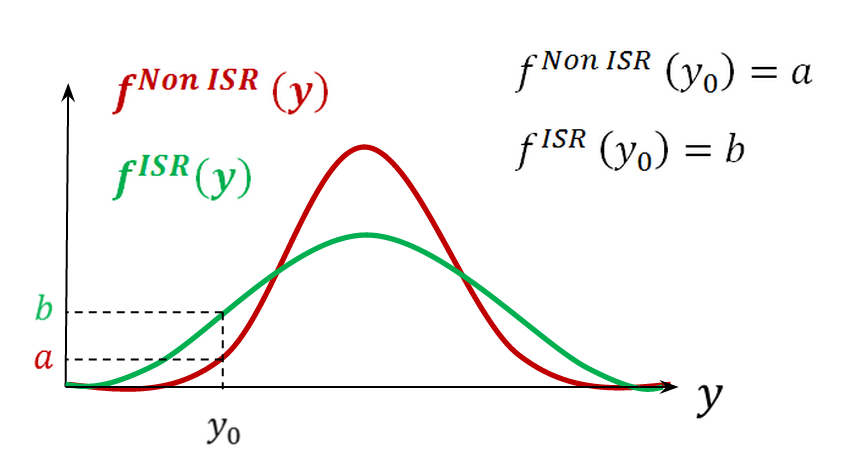
\includegraphics[width=0.5\linewidth]{./Imags_Doc/Prob_ISR_Non}
	\caption[Probability distributions ISR - Non ISR]{Probability distributions of a variable that distinguishes between ISR and Non ISR jets}
	\label{fig:Prob_ISR_Non}
\end{figure}

The difference between both distributions could be used to write the probability of such jet being
ISR or not. In fact, the probability of being ISR should be proportional to the ISR distribution
function at the measurement. Likewise, the probability of being non ISR should be proportional to
the Non ISR distribution function:

\begin{equation} \label{eq:Prob_ISR_1}
P^{ISR}(y_0) \propto f^{ISR}(y_0),
\end{equation}
\begin{equation} \label{eq:Prob_Non_ISR_1}
P^{Non\ ISR}(y_0) \propto f^{Non\ ISR}(y_0).
\end{equation}

In addition to the information offered by the density functions, another important 
consideration to take into account is the \textit{apriori} probability of being ISR. If just one
jet of the $ N_{jets} $ in the event is ISR, the \textit{apriori} probability of any jet being ISR is:

\begin{equation} \label{eq:Prob_ISR_2}
P^{ISR}_{apriori}(y_0) = \frac{1}{N_{jets}},
\end{equation}

\noindent and similarly, the \textit{apriori} probability of any jet being Non ISR is:

\begin{equation} \label{eq:Prob_Non_ISR_2}
P^{Non\ ISR}_{apriori}(y_0) = \frac{N_{jets}-1}{N_{jets}}.
\end{equation}

Combining both assumptions, the probabilities of being ISR and Non ISR could be written as:

\begin{equation} \label{eq:Prob_ISR_3}
P^{ISR}(y_0) = \alpha f^{ISR}(y_0) \frac{1}{N_{jets}},
\end{equation}
\begin{equation} \label{eq:Prob_Non_ISR_3}
P^{Non\ ISR}(y_0) = \alpha f^{Non\ ISR}(y_0) \frac{N_{jets}-1}{N_{jets}},
\end{equation}

\noindent where $ \alpha $ is a constant that results from the normalization of the probabilities:

\begin{equation} \label{eq:Normalization}
1 = P^{ISR}(y_0) + P^{FSR}(y_0),
\end{equation}
\begin{equation} \label{eq:alpha}
\alpha = \dfrac{N_{jets}}{f^{ISR}(y_0)+(N_{jets}-1)f^{Non\ ISR}(y_0)}.
\end{equation}

If there are more than a single variable which differentiate between ISR and Non ISR jets, 
the previous analysis can be extended easily. In fact, it is enough to replace de single 
variable probability density functions by multidimensional probability densities. The formulas 
would take the same form as the probability density distributions are scalar functions, 
regardless they depend on a single variable $ y $ or on a vector $ \vec{y} $. Therefore, in 
a multidimensional case, the formulas would be:

\begin{equation} \label{eq:Prob_ISR_vec}
P^{ISR}(\vec{y_0}) = \alpha f^{ISR}(\vec{y_0}) \frac{1}{N_{jets}},
\end{equation}
\begin{equation} \label{eq:Prob_Non_ISR_vec}
P^{Non\ ISR}(\vec{y_0}) = \alpha f^{Non\ ISR}(\vec{y_0}) \frac{N_{jets}-1}{N_{jets}},
\end{equation}

\subsection{From probability density functions to normalized histograms} \label{sec:Histos}

As the latter formulas show, the probabilities of each jet depend on the probability density 
distributions. In practical matters, these functions are replaced by normalized histograms whose 
entries are collected from simulations where the ISR jet is known. 

However, the replacement is just an approximation because a bin of the histogram does not correspond
exactly to the value of the probability density function. Instead, the histogram results from an
integration of the probability distribution:

\begin{equation} \label{eq:histo}
H(y_i) = \int_{\Omega_i} f(y)dy,
\end{equation}

\noindent where $ \Omega_i $ is the range of the bin, as it is presented in Fig. \ref{fig:Histo_shape}.

\begin{figure}[h]
	\centering
	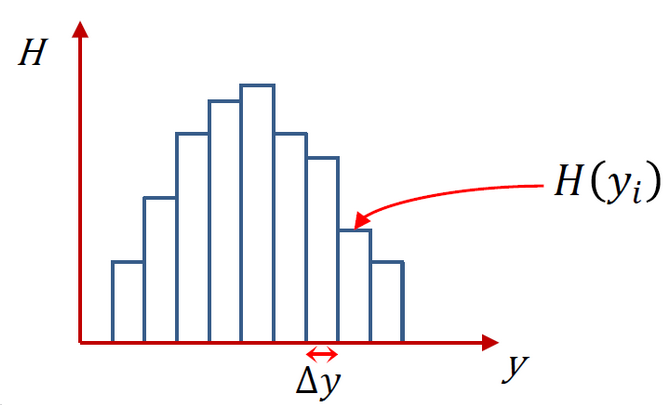
\includegraphics[width=0.5\linewidth]{./Imags_Doc/Histo_shape}
	\caption[Shape of a histogram]{Shape of a histogram which does not exactly correspond with the
		probability density function}
	\label{fig:Histo_shape}
\end{figure}

If the size of the bin is small enough, the expression \ref{eq:histo} can be approximated by:

\begin{equation} \label{eq:Approx_histo}
H(y_i) \approx f(y_i)\Delta y,
\end{equation}

Using this approximation, the practical expressions of the probabilities of being ISR or Non ISR are:

\begin{equation} \label{eq:Prob_ISR_hist}
P^{ISR}(\vec{y_0}) = \alpha H^{ISR}(\vec{y_0}) \frac{1}{N_{jets}},
\end{equation}
\begin{equation} \label{eq:Prob_Non_ISR_hist}
P^{Non\ ISR}(\vec{y_0}) = \alpha H^{Non\ ISR}(\vec{y_0}) \frac{N_{jets}-1}{N_{jets}}.
\end{equation}

To sum up, the usage of these formulas implies the necessity of running 
simulations of several events (with the scheme of chapter \ref{cha:Simulation_chain}),
identifying theoretically the ISR jet in each event, and filling a N-dimensional histogram
for each type of jet (Non ISR and ISR).

\subsection{The Algorithm} \label{sub:Algorithm}

Once the method has been prepared by selecting the distinguishing variables and 
by filling the histograms, the algorithm of Fig. \ref{fig:Tagging_algorithm} 
is applied for each event. First, each jet in the event is studied and its
probabilities of being ISR and Non ISR are determined from
its kinematical variables and expressions \ref{eq:Prob_ISR_vec} and \ref{eq:Prob_Non_ISR_vec}.

\begin{figure}[h]
	\centering
	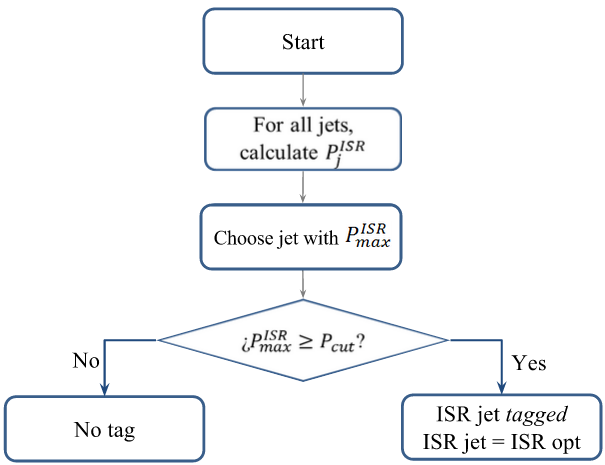
\includegraphics[width=0.8\linewidth]{./Imags_Doc/Tagging_algorithm}
	\caption[ISR jet tagging algorithm]{ISR jet tagging algorithm}
	\label{fig:Tagging_algorithm}
\end{figure}

Then, the jet with greatest probability of being ISR $ P^{ISR}_{max} $ is selected as ISR candidate.
Finally, $ P^{ISR}_{max} $ is compared to a certain cut $ P_{cut} $, in order to ensure that the
algorithm is conclusive. For example, if $ P^{ISR}_{max} < 1/N_{jets} $, the probability of the
ISR candidate is fewer than the \textit{apriori} probability, and therefore no tag should be
imposed. The cut is written in terms of a variable $ k $ that corresponds to the minimum factor
that the probability of the ISR candidate should be greater than the \textit{apriori} probability:

\begin{equation} \label{eq:Prob_cut}
P_{cut} = \frac{k}{N_{jets}}
\end{equation}

This way, the ISR jet is tagged in each event based exclusively on preliminary histograms and 
simple probability considerations.

\subsection{The code}\label{sub:Tagging_code}

The tagging code is presented in Appendix \ref{App:Tagging_code} and in the repository 
of the project, at the folder \texttt{Codes/Codes\_analysis/ISR\_tagging\_FV}. To compile
it, follow the instructions of section \ref{sec:Preparation_codes}. After compilation,
the code can be executed by typing the instruction:

\texttt{./ISR\_tagging [N1] [N2] [N3] [pt\_cut] [k\_cut]}

\noindent where all the parameters that follow \texttt{./ISR\_tagging} are optional. Because
the method uses three kinematic variables to distinguish ISR jets from Non ISR jets,
the last three parameters correspond to the number of the variables the user wants 
for the analysis. There are eight possible variables defined in the program, that can 
be checked in the documentation at the beginning of the code. Although optional, the 
user cannot specify just one or two of them; it is important to execute the code by 
typing the three numbers or none of them. If no variables are written as inputs,
the code takes by default the variables 0, 1 and 2.

On the other hand, the last two variables are used to perform an analysis of the 
tagging results. After executing the tagging algorithm with a probability cut 
\texttt{k\_cut}, a selection of the tagged ISR jets is done by choosing those jets
whose PT is larger than \texttt{pt\_cut}. The performance of the algorithm is 
measured for this selection and plots of Missing Transverse Energy are generated.

Other important parameters of this code are the global variables mentioned in
section \ref{sec:Preparation_codes}. You can change them according to the
rules presented before and compile the code again to use those modifications.
Additionally, the tagging code allows the analysis of several runs, which
is possible to control by means of the \textit{for} loop of line 254.

Other technical details of the tagging program can be found in the comments of 
the code.


\begin{center}
	***
\end{center}

In order to execute the \textit{tagging} algorithm, it is important to prepare
it. That is, it is necessary to fill first the N-dimensional histograms. Therefore,
in addition to the code corresponding to the \textit{tagging} algorithm, other
three codes were written to prepare the \textit{tagging}: \textit{Matching algorithm,
ISR jet analysis} and \textit{Histograms' creation}. In the next sections,
these codes and their functionalities will be presented.

\section{Matching algorithm}\label{sec:Matching}

Some pages above, it was said that the success of the \textit{tagging} algorithm
is based on the information contained by the N-dimensional histograms.
Naturally, those histograms need to be filled with events
where the ISR jet is known. Because Delphes reports the results as the 
experiment does, the kinematic variables of the histograms should be taken
from jets reported by Delphes, which implies the necessity of knowing the ISR
jet at the Delphes simulation stage.

However, the ISR emission is done by Pythia, which introduces ISR partons and
hadronizes them. Only the final particles that result from the hadronization are 
taken by Delphes in order to simulate the detector and thus, it is impossible 
to know the \textquoteleft theoretical' ISR jet with the Delphes simulation exclusively. 
Therefore, it is necessary to \textit{match} \footnote{We have called this procedure 
\textit{matching}. Please do not confuse it with the algorithm carried out
between MadGraph and Pythia, that has been mentioned in chapter \ref{cha:Simulation_chain} ~\cite{matching}.} the ISR parton from Pythia with 
one of the jets from Delphes. Observe that this is a computational procedure 
that cannot be done with real data; it is only useful to identify the ISR jet 
in Delphes and then to fill the N-dimensional histograms.

\begin{figure} [h!]
\centering
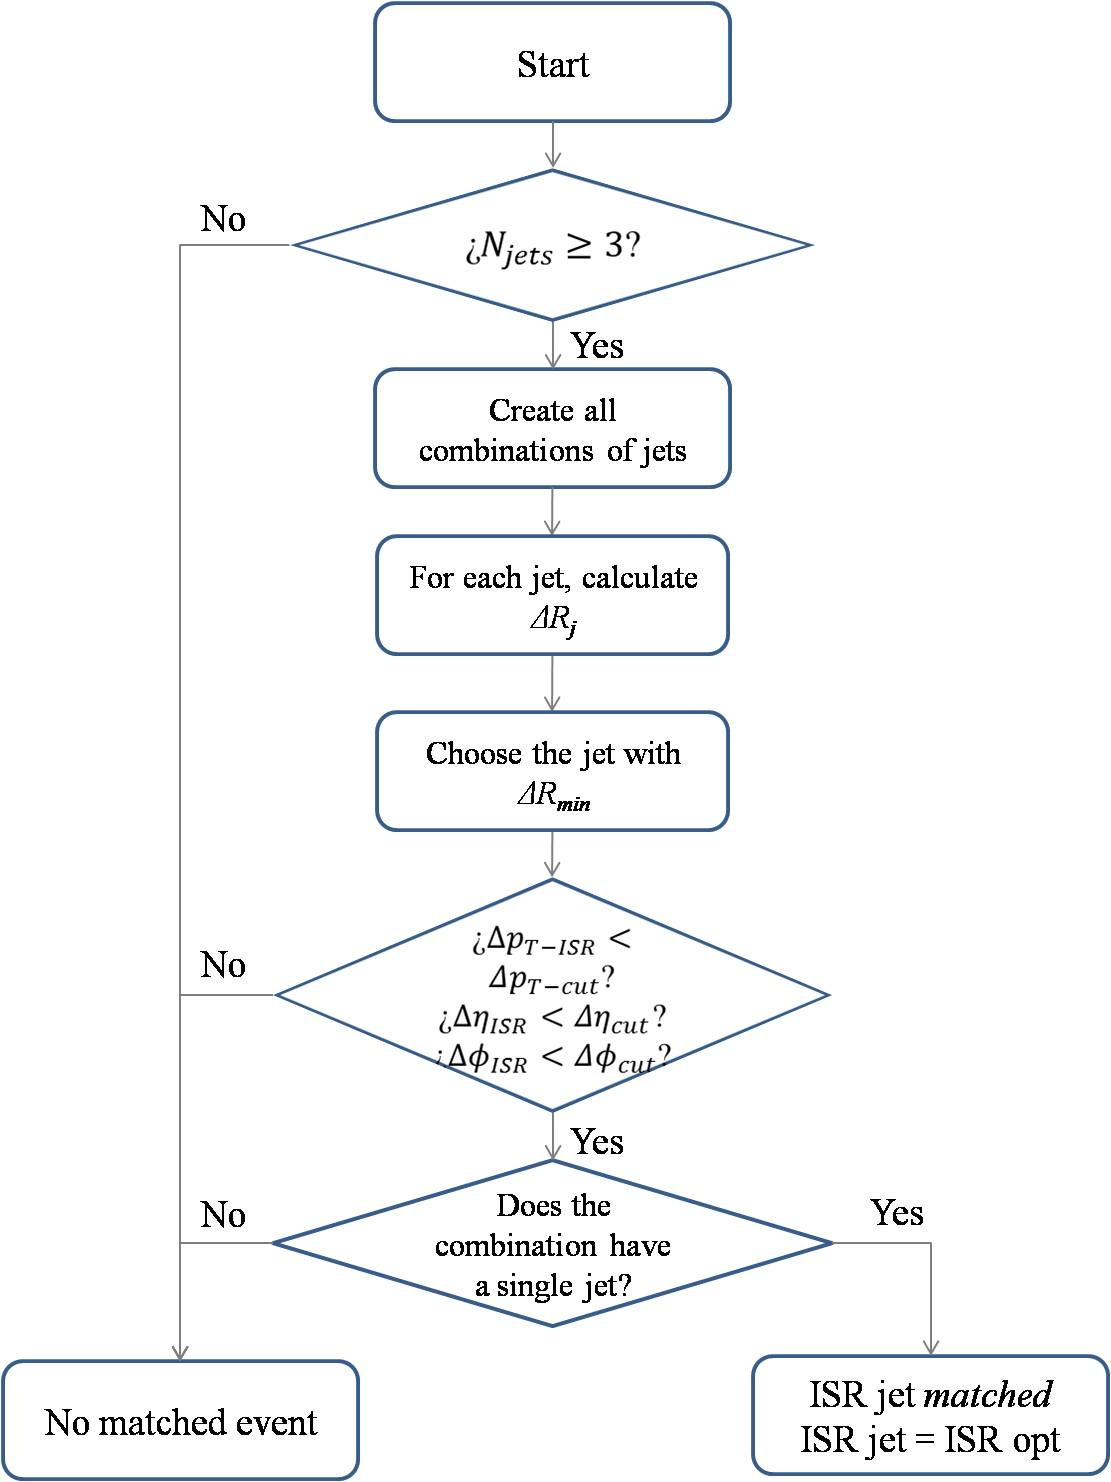
\includegraphics[width=0.7\linewidth]{./Imags_Doc/Matching_algorithm}
\caption[Matching algorithm]{Matching algorithm between MadGraph and Pythia}
\label{fig:Matching_algorithm}
\end{figure}

The \textit{matching} algorithm is presented in Fig. \ref{fig:Matching_algorithm}.
In practical matters, after knowing the ISR parton in Pythia, it looks for the
closest jet using the cone-algorithm. It not only considers the jets reported
by Delphes, but also combinations between them (i.e. up to three of them). This
considers the case when a parton results in more than a single jet because of 
the detector interpretation. After choosing the closest jet (or combination) to
the ISR parton, the algorithm ensures that the optimum jet is inside a reasonable
region around the ISR parton. If the matched jet is too far from the ISR parton
or if it is a combination of several jets, the method does not report any 
match as it is shown in the last two boxes of scheme \ref{fig:Matching_algorithm}.

As in the case of the tagging algorithm, follow the instructions of section
\ref{sec:Preparation_codes} to compile and modify the global variables of
the code, which can be found in Appendix \ref{App:Matching_code} and in the
repository of the project. Once the code has been compiled, it can be executed
by typing the instruction:

\texttt{./ISR\_matching [000]}

where the last three digits are optional and correspond to the number of the
simulation (its seed) to which the user wants to execute the matching. If no
parameter is written, the simulation for analysis has seed 003.

Observe that in contrast with the tagging code, the matching code does not 
execute the algorithm for several runs but only one. In consequence, a script 
has been  written in order to perform several matching procedures. This script,
called \texttt{script\_several\_matchings.sh}, is available in the repository
(in the same folder of the matching code). In order to use it, modify line 8 
according to the simulations to which you want to perform the matching and then,
type the instruction:

\texttt{./script\_several\_matchings.sh} \footnote{Possibly, it is necessary
	to change the permissions of this script to execute it. Type \texttt{chmod
		a+x script\_several\_matchings.sh} to do so.}

As a result of executing the matching algorithm, a binary file containing a
list with the ISR partons is generated. For those events without matching,
the entry of the list is $ -1 $. The file, with name \texttt{ISR\_jetssTops\_WI\_005.bn}
\footnote{Check the structure of the name in section \ref{sec:Preparation_codes}},
is used as input by the other codes to know which is in \textquoteleft 
theory' the ISR jet.

Finally, more documentation can be found in the comments of the code.

\section{ISR jet analysis code} \label{sec:ISR_analysys}

Several times throughout the project, it was necessary to compare ISR jets
and Non ISR jets. The comparison between both kind of jets allowed the
subsequent selection of the suitable variables for the execution of 
the tagging algorithm. Due to this importance, a separate code was written
in order to develop such comparison. Again, the code can be found in 
Appendix !!-\_/-!!  and in the repository of the project, in the folder \texttt{Codes/Codes\_analysis/ ISR\_jet\_analysis\_FV}.

The program takes as inputs a group of simulations and their corresponding
matching results. Then, it creates histograms of kinematic variables 

\begin{appendices}

\chapter[Simulation codes]{Simulation codes and scripts}\label{App:Simulation_codes}
\section[Pythia code]{Pythia code: hadronization02.cc}\label{App:hadronization02.cc}
\lstinputlisting[language=C++]{Codes/hadronization02.cc}
\newpage
\section[Integration scripts]{Integration scripts: MadGraph + Pythia + Delphes}\label{App:scripts}
\subsection{Configuration script: \texttt{config\_Integration.ini}}\label{sub:Configuration_script}
\lstinputlisting[language=bash]{Codes/config_Integration.ini}
\subsection{Execution script: \texttt{script\_Integration.sh}}\label{sub:Execution_script}
\lstinputlisting[language=bash]{Codes/script_Integration.sh}

\chapter[Analysis codes]{Analysis codes}\label{App:Analysis_codes}
\section[Tagging algorithm]{Tagging algorithm}\label{App:Tagging_code}
\lstinputlisting[language=C++]{Codes/ISR_tagging.cpp}
\section[Matching algorithm]{Matching algorithm}\label{App:Matching_code}
\lstinputlisting[language=C++]{Codes/ISR_matching.cpp}

\end{appendices}


\bibliographystyle{unsrt}

\bibliography{My_Bibliography_report}\addcontentsline{toc}{chapter}{Bibliography}
	

\end{document}
